%%%%%%%%%%%%%%%%%%%%%%%%%%%%%%%%%%%%%%%%%%%%%%%%%%%%%%%%%%
%
% Doctoral Thesis Template @ The University of Manchester
% LaTeX Chapter Template
% Version 1 (23/07/2020)
% Joe Crone
%
% This template is based on:
% The University of Manchester, Presentation of Thesis Policy
% Research Office Graduate Education Team
% June 2017
% http://www.regulations.manchester.ac.uk/pgr-presentation-theses/
%
%%%%%%%%%%%%%%%%%%%%%%%%%%%%%%%%%%%%%%%%%%%%%%%%%%%%%%%%%%
\documentclass[../main.tex]{subfiles}
\begin{document}

% Title
%--------------------------------------------------------
\chapter{CBETA Inverse Compton Source Design}
\label{CBETA_Inverse_Compton_Source_Design} % to reference use \ref{ChapterTemplate}

\begin{figure}
\centering
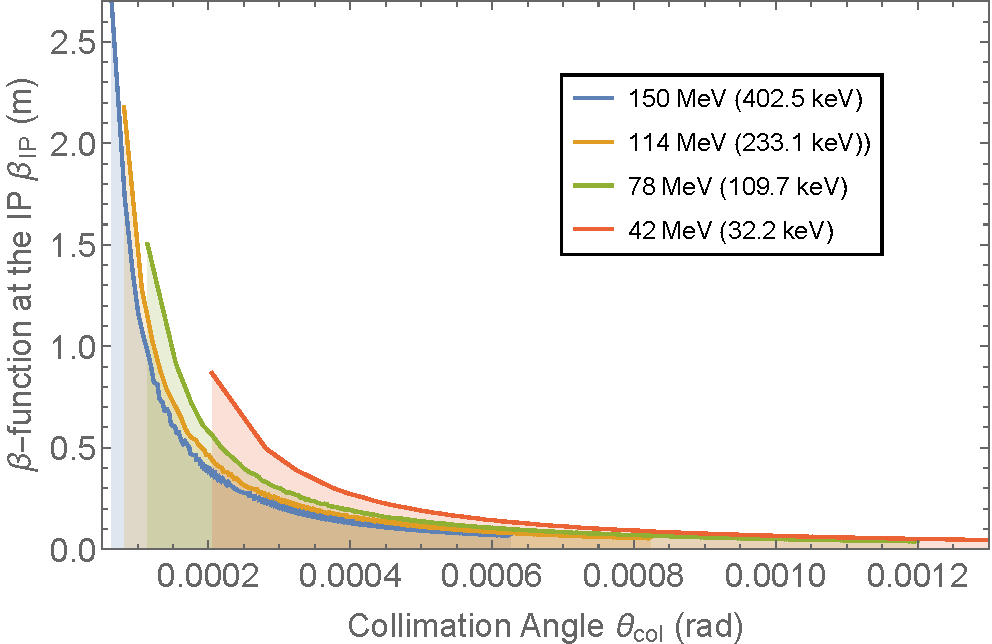
\includegraphics[width=0.8\textwidth]{Figures/CBETA_Inverse_Compton_Source_Design/CBETABetaTheta.pdf}
\caption{Tuning curves of $\beta^{*}$ against $\theta_{\mathrm{col}}$ for each of the nominal CBETA electron beam energies satisfying the maximal flux across the 0--1\% bandwidth range. Minimised bandwidth solutions in this range have large $\beta$-functions at the IP and small collimation angles $\theta_{\mathrm{col}}$; the maximal bandwidth solutions have small $\beta$-functions and larger collimation angles $\theta_{\mathrm{col}}$.\textcolor{blue}{**THIS SHOULD BE REPLACED BY ONE FROM NEW CODE WITH LESS NOISE**}}
\label{fig:CBETA_beta_theta_parameter_space}
\end{figure}


\begin{figure}[!htb]
\centering
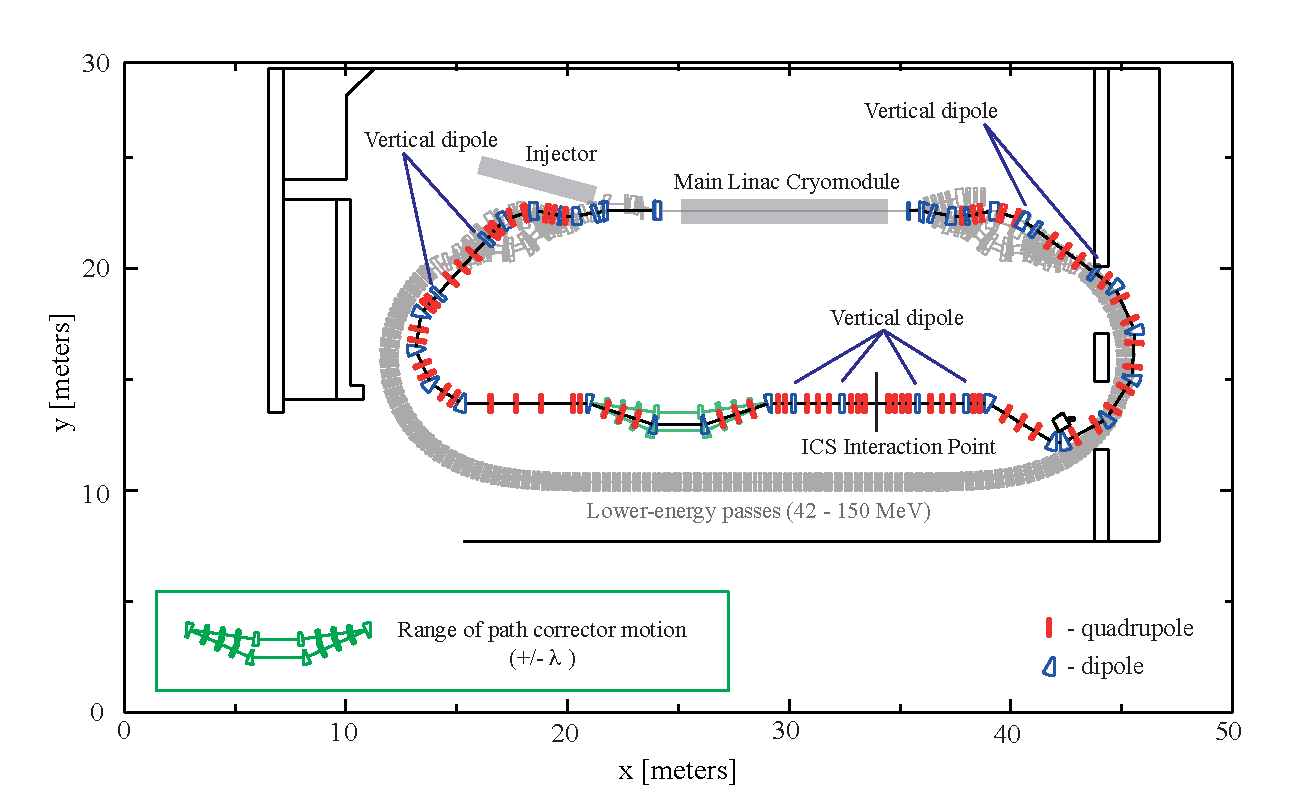
\includegraphics[width=\textwidth]{Figures/CBETA_Inverse_Compton_Source_Design/cbetaicslayout.pdf}
\caption{Layout of the ICS bypass in CBETA; greyed beamline elements are already installed in the existing accelerator. Outer walls and relevant existing infrastructure shown in black.}
\label{fig:CBETA_ICS_Layout}
\end{figure}

\begin{figure}[!htb]
    \centering
    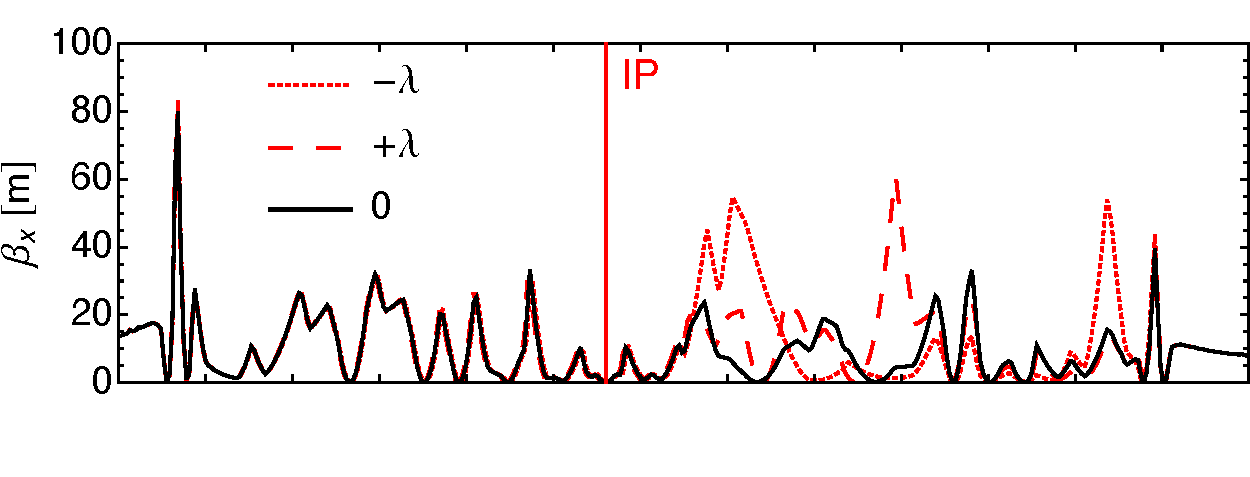
\includegraphics[width=0.8\textwidth]{Figures/CBETA_Inverse_Compton_Source_Design/twissplotx.pdf}
    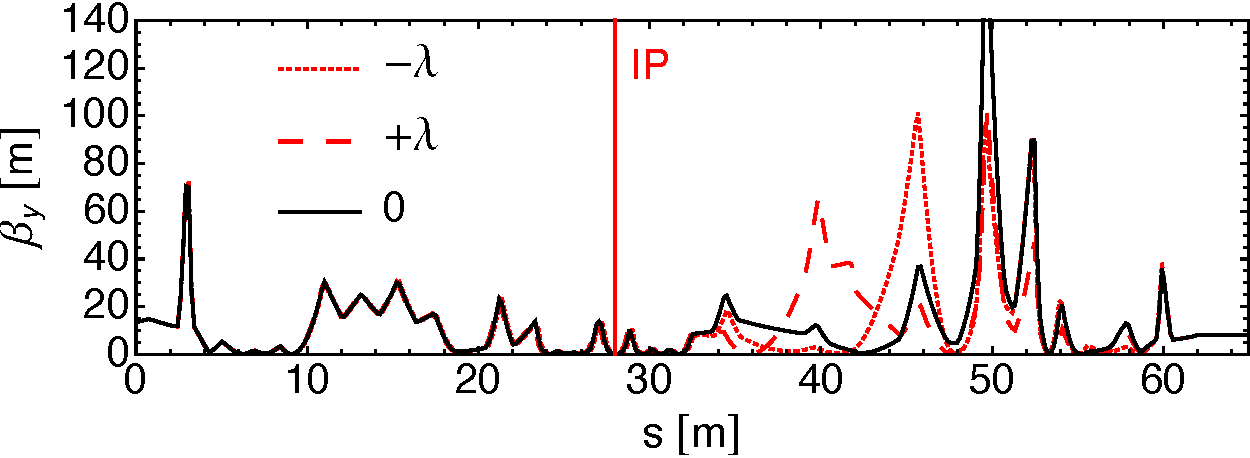
\includegraphics[width=0.8\textwidth]{Figures/CBETA_Inverse_Compton_Source_Design/twissploty.pdf}
    \caption{Twiss functions in the ICS bypass line, showing the re-matched conditions for different path length configurations $-\lambda_{RF}$, $0$ and $+\lambda_{RF}$. The ICS interaction point (IP) is indicated.}
    \label{fig:CBETA_ICS_Twiss}
\end{figure}

\begin{figure}[!htb]
\centering
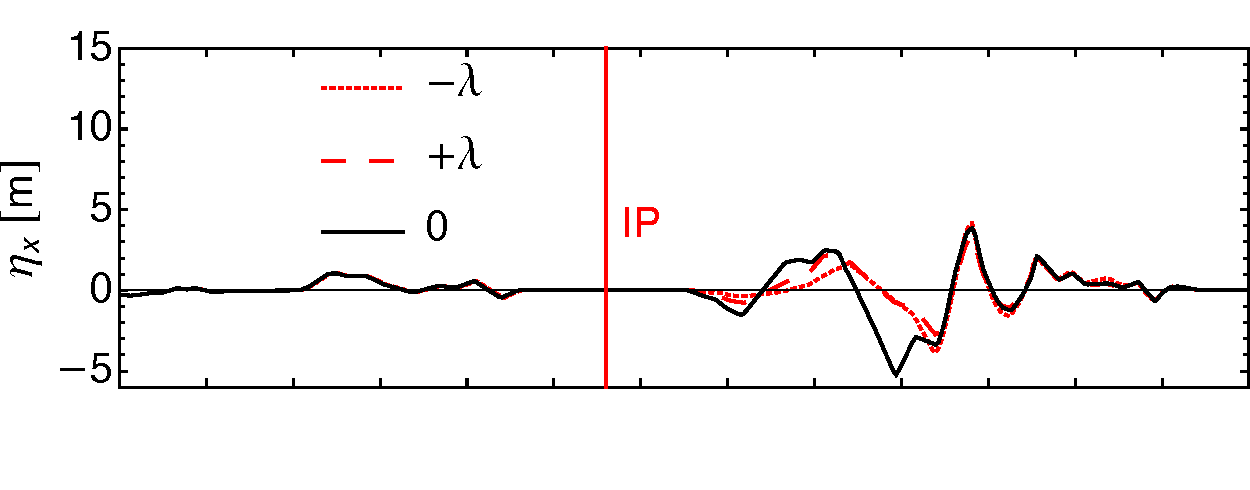
\includegraphics[width=0.8\textwidth]{Figures/CBETA_Inverse_Compton_Source_Design/dispplotx.pdf}
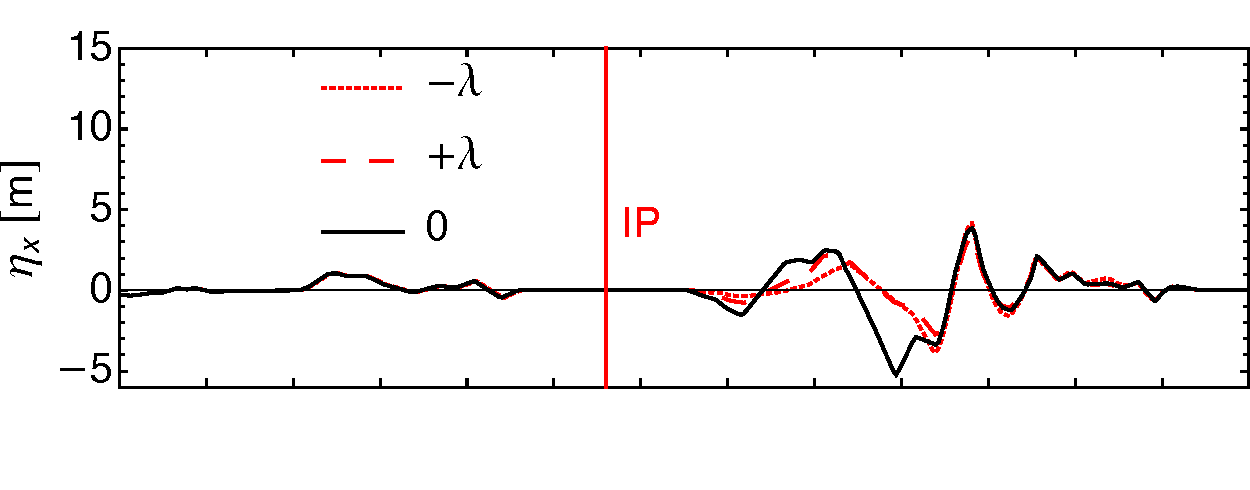
\includegraphics[width=0.8\textwidth]{Figures/CBETA_Inverse_Compton_Source_Design/dispplotx.pdf}
\caption{Dispersion functions in the ICS bypass line for the 0.5\% bandwidth case, showing the re-matched conditions for different path length configurations $-\lambda_{RF}$, $0$ and $+\lambda_{RF}$. The ICS interaction point (IP) is indicated.}
\label{fig:CBETA_ICS_dispersion}
\end{figure}

Predicted spectral output (flux) from 1064~nm photons colliding head-on with the $E_e =150$~MeV (kinetic energy) electrons in CBETA; this spectrum was generated using the \textsc{ICCS3D} code, and is consistent with calculations using the method of Sun et al. This spectrum has a peak energy of 403.3~keV; using the proposed 5~degree crossing angle, the peak energy is reduced to 402.5~keV and the spectral density is reduced by a factor $\sim$~5.

\begin{figure}
\centering
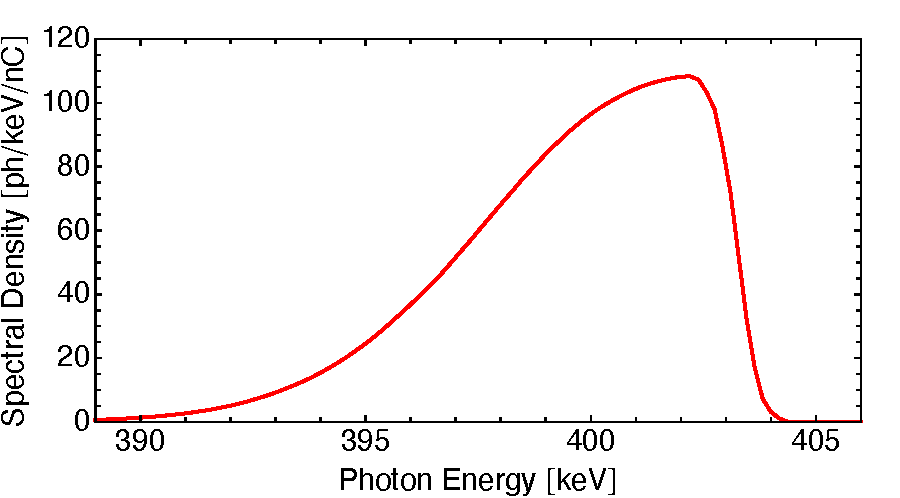
\includegraphics[width=0.8\textwidth]{Figures/CBETA_Inverse_Compton_Source_Design/cbetaspectrumplot.pdf}
\caption{Predicted spectral output (flux) from 1064~nm photons colliding head-on with the $E_e =150$~MeV (kinetic energy) electrons in CBETA; this spectrum was generated using the \textsc{ICCS3D} code, and is consistent with calculations using the method of Sun et al. This spectrum has a peak energy of 403.3~keV; using the proposed 5~degree crossing angle, the peak energy is reduced to 402.5~keV and the spectral density is reduced by a factor $\sim$~5.}
\label{fig:my_label}
\end{figure}

\begin{figure}
\centering
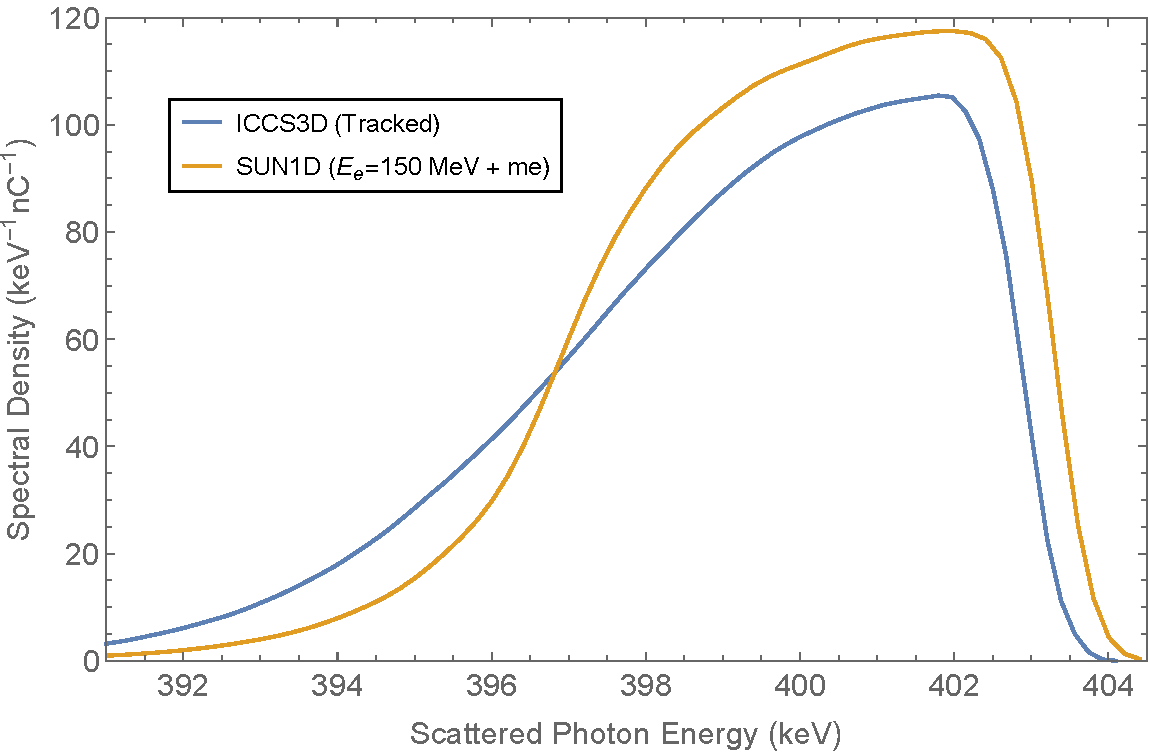
\includegraphics[width=0.8\textwidth]{Figures/CBETA_Inverse_Compton_Source_Design/CBETAICSSpectra.pdf}
\caption{caption}
\label{fig:CBETA_ICS_Spectra}
\end{figure}

\begin{figure}
\centering
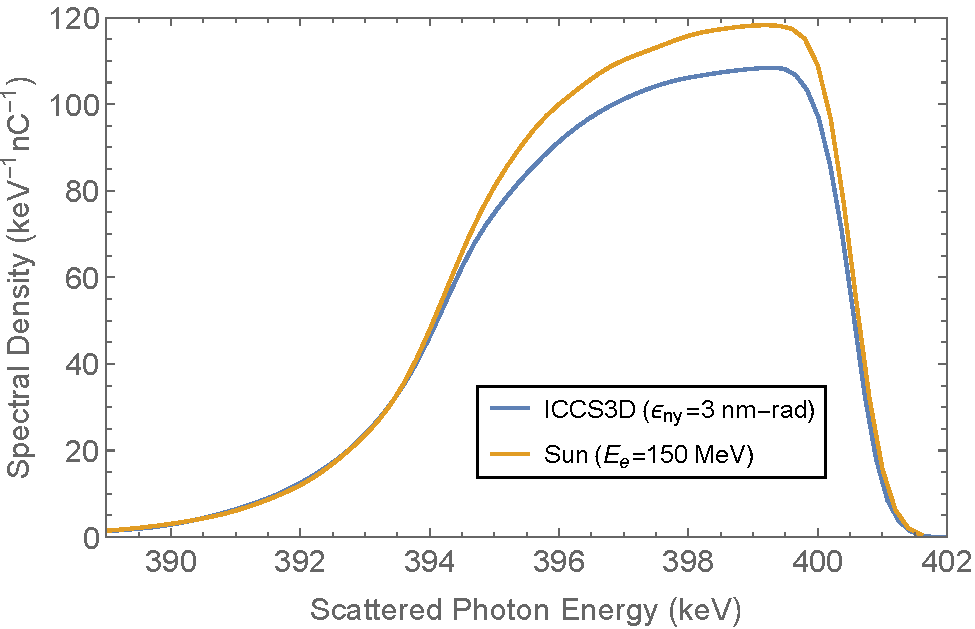
\includegraphics[width=0.8\textwidth]{Figures/CBETA_Inverse_Compton_Source_Design/150MeVBenchmarkSpectra.pdf}
\caption{Caption}
\label{fig:CBETA_Benchmarking_Spectra}
\end{figure}

\end{document}